\documentclass[
10pt, % Set the default font size, options include: 8pt, 9pt, 10pt, 11pt, 12pt, 14pt, 17pt, 20pt
%
aspectratio=169, % Uncomment to set the aspect ratio to a 16:9 ratio which matches the aspect ratio of 1080p and 4K screens and projectors
]{beamer}

\usepackage{etoolbox}
\usepackage[utf8]{inputenc}

\usepackage{mathtools}
\usepackage{amsmath}
\usepackage{pgfplots}
\usepackage{dsfont}
\usepackage{faktor}
\usepackage{ latexsym }
\usepackage{amssymb }
\usepackage{xcolor}
\usepackage{colortbl}
\usepackage{array}

\usepackage{fontawesome5}
\usepackage{MnSymbol,wasysym} %Pour des smileys

\usepackage{multirow,bigdelim}
\usepackage{multicol}

\usepackage[framemethod=default]{mdframed}
\usepackage{pifont}

\newcolumntype{C}[1]{>{\centering\let\newline\\ \arraybackslash\hspace{0pt}}m{#1}}

\usefonttheme[onlymath]{serif} %De belles formules
\usepackage{xcolor}


\newcommand\F{\mathbb{F}}
\newcommand\Fq{\mathbb{F}_q}
\newcommand\Fqm{\mathbb{F}_{q^m}}
\newcommand\Z{\mathbb{Z}}
\newcommand\A{\mathbb{A}}
\newcommand\PP{\mathbb{P}}
\newcommand\N{\mathbb{N}}
\newcommand\T{\mathbb{T}}
\newcommand\R{\mathbb{R}}

\newcommand{\calC}{\mathcal{C}}
\newcommand{\calD}{\mathcal{D}}
\newcommand{\calF}{\mathcal{F}}
\newcommand{\calH}{\mathcal{H}}
\newcommand{\calL}{\mathcal{L}}
\newcommand{\calP}{\mathcal{P}}
\newcommand{\calR}{\mathcal{R}}
\newcommand{\calX}{\mathcal{X}}
\newcommand{\calY}{\mathcal{Y}}

\newcommand\bfc{\vec{c}}
\newcommand\bfd{\vec{d}}
\newcommand\bfm{\vec{m}}
\newcommand\bfx{\vec{x}}
\newcommand\bfy{\vec{y}}
\newcommand\bfz{\vec{z}}


\newcommand\RS{\mathsf{RS}}
\newcommand\GRS{\mathsf{GRS}}
\newcommand{\set}[1]{\left\{#1\right\}}

\renewcommand{\vec}[1]{\boldsymbol{#1}}

\newcommand{\ps}[2]{\left\langle #1,#2 \right\rangle}
\renewcommand{\epsilon}{\varepsilon}

\DeclareMathOperator{\ev}{ev}
\DeclareMathOperator{\Span}{Span}
\DeclareMathOperator{\Supp}{Supp}
\DeclareMathOperator{\Tr}{Tr}
\newcommand{\degab}[1]{\deg_{a,b}\left(#1\right)}


% Bien aligner ses incides multi-lignes

\makeatletter
\newcommand{\subalign}[1]{%
	\vcenter{%
		\Let@ \restore@math@cr \default@tag
		\baselineskip\fontdimen10 \scriptfont\tw@
		\advance\baselineskip\fontdimen12 \scriptfont\tw@
		\lineskip\thr@@\fontdimen8 \scriptfont\thr@@
		\lineskiplimit\lineskip
		\ialign{\hfil$\m@th\scriptstyle##$&$\m@th\scriptstyle{}##$\hfil\crcr
			#1\crcr
		}%
	}%
}
\makeatother


\mdfdefinestyle{mdf}{innerleftmargin=0.3em,innerrightmargin=0.3em,innertopmargin=0.3em,innerbottommargin=0.3em,linecolor=white}





%-----Commandes Beamer %-----------------------

\DeclareOptionBeamer{compress}{\beamer@compresstrue}
\ProcessOptionsBeamer

\mode<presentation>

\useoutertheme[footline=authortitle, footline=frame number,subsection=false]{miniframes}
\useinnertheme{circles}
\usecolortheme{whale}
\usecolortheme{orchid}

\definecolor{beamer@blendedblue}{rgb}{0.137,0.466,0.741}

\setbeamercolor{structure}{fg=black}
\setbeamercolor{titlelike}{parent=structure}
\setbeamercolor{frametitle}{bg=structure!70,fg=white}
\setbeamerfont{frametitle}{size=\small,series=\bfseries}
\setbeamercolor{title}{fg=black}
\setbeamercolor{item}{fg=black}
\setbeamertemplate{page number in head/foot}[totalframenumber] %Pour ajouter le numéro des slides
\setbeamerfont{block title}{size=\small,series=\bfseries}

\setbeamercolor{block title example}{fg=white,bg=teal}
\setbeamercolor{block body example}{fg=black,bg=teal!10}


\setbeamercolor{block title alerted}{fg=white,bg=red!45!yellow}
\setbeamercolor{block body alerted}{fg=black,bg=red!40!yellow!10}


\setbeamertemplate{frametitle}{%
	\nointerlineskip%
	\begin{beamercolorbox}[wd=\paperwidth,ht=2.0ex,dp=0.6ex]{frametitle}
		\hspace*{1ex}\insertframetitle%
	\end{beamercolorbox}%
}

%Pour mettre les miniframes (ronds) sur la même ligne que ls sections
\makeatletter
\patchcmd{\slideentry}{\advance\beamer@tempdim by -.05cm}{\advance\beamer@tempdim by\beamer@vboxoffset\advance\beamer@tempdim by\beamer@boxsize\advance\beamer@tempdim by 1.2\pgflinewidth}{}{}
\patchcmd{\slideentry}{\kern\beamer@tempdim}{\advance\beamer@tempdim by 2pt\advance\beamer@tempdim by\wd\beamer@sectionbox\kern\beamer@tempdim}{}{}
\makeatother

\mode<all>
%\includeonlyframes{current}

\setbeamersize{text margin left=0.8cm,text margin right=0.8cm}

\setbeamertemplate{navigation symbols}{}  %Bye bye les boutons du bas

%----------------Espaces autour équations%---------

\makeatletter
\g@addto@macro\normalsize{%
	\setlength\belowdisplayskip{0.2em}
	\setlength\abovedisplayskip{0.2em}
}

%----------------


\vfuzz=25pt %Evite les alertes "Over full \vbox" jusqu'à 25pt.

%---------------- Tikz Packages ------------------
\usepackage{tikz}
\usetikzlibrary{tikzmark} %Permet de créer des noeuds dans du texte pour annoter dans un tikz ultérieur. Très pratique pour annoter les formules moches.
\usetikzlibrary{arrows,patterns,positioning,fit}
\usetikzlibrary{matrix,arrows,shapes,shapes.misc}
\usetikzlibrary{decorations.pathreplacing,angles,quotes}
\usetikzlibrary{decorations.markings,calc}
\usetikzlibrary{overlay-beamer-styles,backgrounds} %Pour utiliser alt dans tikz
\tikzset{>=stealth} % Change le style de flèche dans tikz

%--------- Un bout de code pour récupérer la couleur d'un noeud rectangulaire ou circulaire : noeud.f pour la couleur du fill, noeud.d pour celle du draw ---------------
% Voir https://tex.stackexchange.com/questions/602047/is-obtaining-the-color-of-a-node-possible

\makeatletter
\def\pgf@sh@fbg@circle{%
	\@ifundefinedcolor{pgffillcolor}{}{\xglobal\colorlet{\pgf@node@name.f}{pgffillcolor}}%
	\@ifundefinedcolor{pgfstrokecolor}{}{\xglobal\colorlet{\pgf@node@name.d}{pgfstrokecolor}}%
}
\def\pgf@sh@fbg@rectangle{%
	\@ifundefinedcolor{pgffillcolor}{}{\xglobal\colorlet{\pgf@node@name.f}{pgffillcolor}}%
	\@ifundefinedcolor{pgfstrokecolor}{}{\xglobal\colorlet{\pgf@node@name.d}{pgfstrokecolor}}%
}
\makeatother

%-Après avoir défini un \tikzmarknode{noeuf}{texte}, on crée un noeuf rectangulaire (aux coins arrondis) autour d'une certaine couleur et on annote avec une flèche.

\newcommand\highlightnode[2]{ %args: noeud, couleur
	\node (#1-frame)[rounded corners,fit=(#1),inner sep=2pt,fill=#2,fill opacity=0.17] {};
}

\newcommand\framenode[6][(0,0)]{ %args: (shift) noeud, position, couleur, texte , booléen flèche 0 = non / 1 = oui
	\highlightnode{#2}{#4}
	\node [#2-frame.f,#3 of = #2, shift={#1}](#2-text){#5};
	\ifx1#6 	\draw[#2-frame.f,<-] (#2-frame) -- (#2-text); \fi		
}

%-----------Couleurs-------------
\colorlet{bgreen}{green!60!black} 
\colorlet{bred}{red!70!black} 
\colorlet{alertcolor}{red!60!yellow}
\renewcommand{\alert}[1]{\textcolor{alertcolor}{#1}}
\newcommand{\new}[1]{\textcolor{blue!60!green}{#1}}
\newcommand{\blue}[1]{\textcolor{beamer@blendedblue!70!black}{#1}}
\newcommand{\rawblue}[1]{\textcolor{blue}{#1}}
\newcommand{\details}[1]{\scalebox{0.8}{\textcolor{structure!20!black!80}{#1}}}







%%%%%%%%%%%%%%%%%%%%%%%%%%%% Title %%%%%%%%%%%%%%%%%%%%%
\title[Goppa-Like AG codes Distinguisher]{\scshape Goppa–Like AG Codes from $C_{a,b}$ curves And the dimension of the square of their dual}
%\subtitle{Subtitle}
\author{Sabira El Khalfaoui, Mathieu Lhotel, \textbf{Jade Nardi}}



\institute[]{CNRS, IRMAR, University of Rennes, France}
\date{$AGC^2T$ 2023\\$9^{th}$ June 2023}

\begin{document}
	
{
		\setbeamertemplate{background} 
		{
			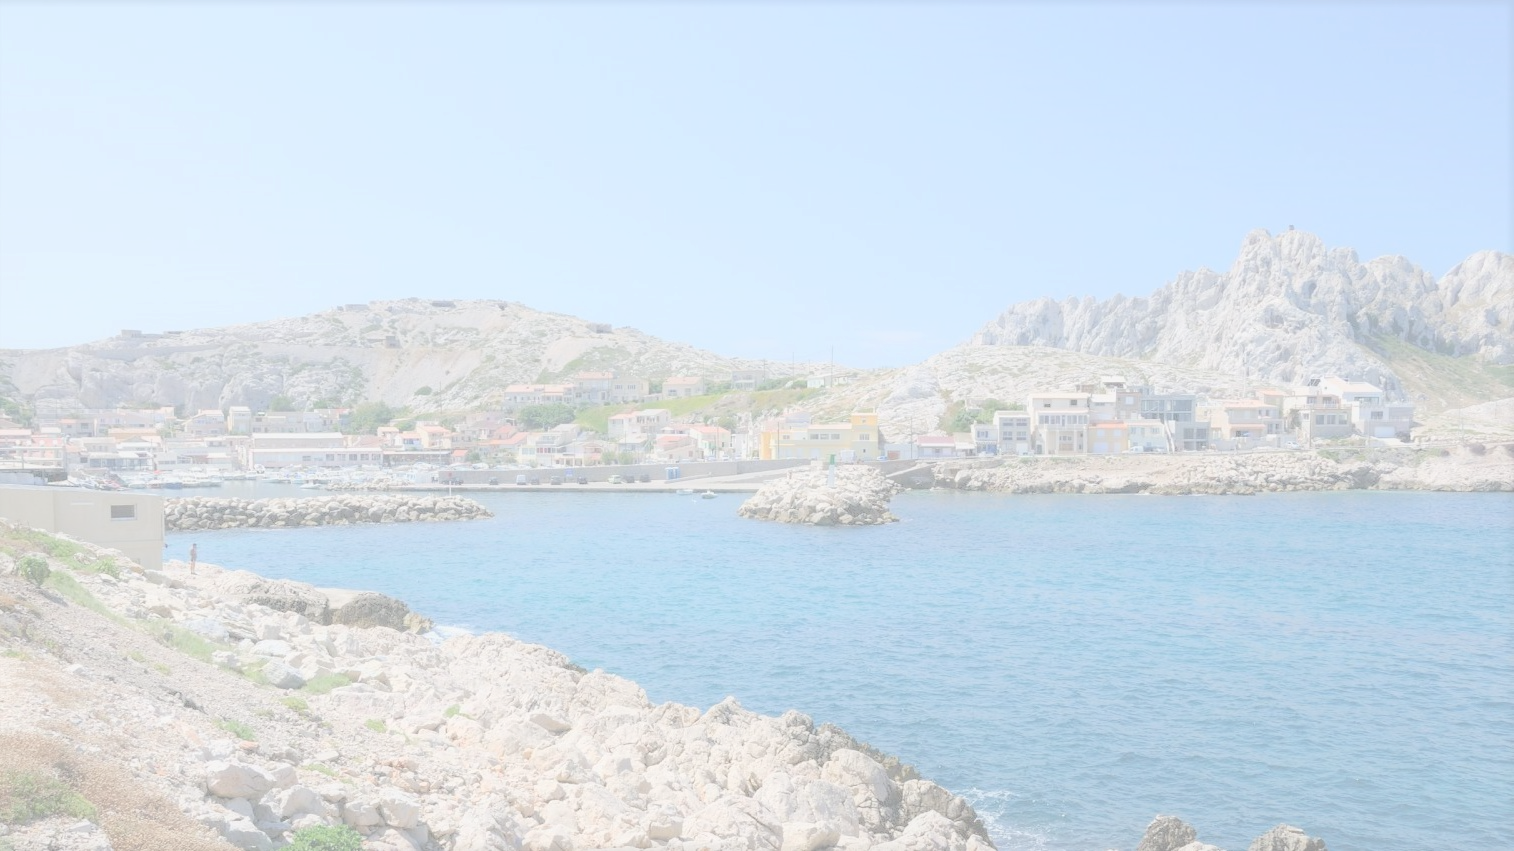
\includegraphics[width=\paperwidth,height=\paperheight]{goudes2}
		}
		
	\begin{frame}[noframenumbering,plain]
	
	\maketitle
	
	\begin{mdframed}[style=mdf,backgroundcolor=white]
		\centering
		\url{arxiv.org/abs/2303.08687}
	\end{mdframed}
	
	\end{frame}%-------------------------------------
}
\section{Linear codes}		
	\begin{frame}
			\frametitle{Preliminaries: linear code}
			Let $q$ be a prime power and $\Fq$ a finite field of size $q$. 
			\begin{block}{Definition: Linear code}
				A \textbf{linear code} $\calC$ of \blue{length $n$} is a vector subspace of $\Fq^n$. It is said to be \blue{$t$--correcting} if $\omega(\bfc) \geq 2t + 1$ for every $\bfc=(c_1,\dots,c_n) \in \calC$, where $\omega(\bfc)= \#\{i \mid c_i \neq 0\}$ \details{(Hamming weight)}.
				
				\smallskip
				
				A \textbf{generator matrix} of $\calC$ is a matrix whose rows form a basis of $\calC$.
			\end{block}
			
			The \textbf{dual code} of $\calC$ is $\calC^{\perp}=\left\lbrace \bfx \in \Fq^n \mid \bfc \cdot \bfx=0, \text{ for all } \bfc \in \calC \right\rbrace$ . \hfill \details{($\cdot$ is the usual scalar product.)}
			
					
\end{frame}
		
		
	\section{McEliece cryptosystem}
		
\begin{frame}
	\frametitle{Context and motivation: McEliece cryptosystem}
	
	$\rightarrow$ First code-based public key encryption (1978).	%was introduced in 1978. 	
	\begin{mdframed}[style=mdf,backgroundcolor=yellow!13]
	\textbf{Parameters:} $n, t \in \N$ with $t \ll n$.
	A family $\calF$ of efficiently decodable $t$--correcting codes $\calC\subset \Fq^n$.
	\end{mdframed}
\vskip0.3em
	\begin{minipage}{0.70\textwidth}
			\begin{mdframed}[style=mdf,backgroundcolor=alertcolor!10]
			\textbf{Key generation :} $\alert{G^{\text{pub}}}=\textcolor{bred}{S}G\textcolor{bred}{P}$ where
			\begin{itemize}
				\item $G$ is a generator matrix of size $k \times n$ of a \textit{random} code $\calC \in\calF$,
				\item \textcolor{bred}{$S$} is a \emph{random} invertible $k \times k$,
				\item \textcolor{bred}{$P$} is a \emph{random} permutation $n \times n$ matrix.
			\end{itemize}
			
		\end{mdframed}
	\end{minipage}\hfill
	\begin{minipage}{0.29\textwidth}
		\begin{mdframed}[style=mdf,backgroundcolor=purple!10]
			\textbf{Public key:} $(\alert{G^{\text{pub}}},t)$.
		\end{mdframed}
	\vskip-0.4em
	\begin{mdframed}[style=mdf,backgroundcolor=blue!8]
			\textbf{Private key:} $(\textcolor{bred}{S},D_\calC,\textcolor{bred}{P})$ where $D_\calC$ is an efficient decoding algorithm for $\calC$.
	\end{mdframed}
	\end{minipage}
	\vskip-0.4em
	\begin{mdframed}[style=mdf,backgroundcolor=green!8]
	\textbf{Encryption of a cleartext $\bfm \in \Fq^k$:} \emph{randomly} pick $\bfz \in \F^n$ of weight $t$. \hfill $\rightarrow$ $\bfy = \bfm \alert{G^{\text{pub}}} + \bfz$.
	\end{mdframed}
	\vskip-0.4em
	\begin{mdframed}[style=mdf,backgroundcolor=blue!70!red!10]
		\textbf{Decryption} using the private key.
	\end{mdframed}
	
	\medskip
	
	\begin{minipage}{0.27\textwidth}
		Its security is based on 
		
		\vspace*{1.5em}
	\end{minipage}%
	\begin{minipage}{0.72\textwidth}
		\begin{enumerate}
		\item the hardness of decoding random linear codes,
		\item the indistinguishability of the chosen codes from random ones.
	\end{enumerate}
	\end{minipage}
	
	

	\bigskip
	
	McEliece's original proposal, based on \textbf{binary Goppa codes}, has \textcolor{bred}{very large key size}.
	
\end{frame}%-------------------------------------
		
		
		
	


\begin{frame}
	\frametitle{Goppa codes}
	
	
	\begin{block}{Definition: \textbf{Generalized Reed--Solomon (GRS)}}
		Let $\bfx=(x_1,\cdots,x_n) \in \Fq^n$  with distinct entries (\textbf{support}) and \textbf{multiplier} $\bfy \in (\Fq^*)^n$.
		\[\GRS_r(\bfx,\bfy)=\{(y_1f(x_1),y_2f(x_2),\dots,y_nf(x_n)) \mid f \in \Fq[X] \text{ such that } \deg f < r \}.\]
	\end{block}
	
	\begin{block}{Definition: Subfield subcode}
		Let $\calC$ be a linear code over $\Fqm$.
		Its \textbf{subfield subcode} $\calC|_{\Fq}$ is defined by $\calC|_{\Fq}=\calC \cap \mathbb{F}_q^n.$
	\end{block}
	
\begin{block}{Definition: Goppa code of order $r$}
	Let $\bfx=(x_1,\cdots,x_n) \in \Fqm^n$ with distinct entries and $g \in \Fqm [x]$ be a polynomial of degree $r$ such that $\forall i, g(x_i)\neq 0$. The \textbf{Goppa code} associated to $(\bfx, g)$ is defined as \[\Gamma_r(\bfx,g)= \GRS_r(\bfx,\bfy)^\perp|_{\Fq},\]
	where $\bfy = (g(x_1)^{-1},\dots,g(x_n)^{-1})$.
\end{block}



Even if Generalized Reed--Solomon are heavily structured, Goppa codes \textit{look like} random codes.



\end{frame}%----------------------------

\section{Schur product/square}

\begin{frame}
	\frametitle{Schur Product and Square code Distinguisher}
	
	Many attemps to replace Goppa codes have been broken by using an operation that endows $\Fq^n$ with an algebra structure, the \alert{Schur product}.
	
	\medskip
		
	In $\Fq^n$ we denote by $\star$ the \textbf{Schur product} $\bfc \star \bfd = (c_1d_1,\cdots,c_nd_n)$.
	%	\begin{block}{Definition: Schur product}
		%		The Schur product of two vectors $\mathbf{a}$,$\mathbf{b} \in \Fqm^n$ is defined as 
		%		\[ \mathbf{a} \star \mathbf{b} := (a_1b_1,\cdots,a_nb_n). \]
		%	\end{block}

\smallskip
	
	The Schur product of two codes $\calC, \calD \subseteq \Fq^n$ is $\mathbf{\calC } \star \mathbf{\calD }= \Span\set{\bfc \star \bfd \mid \mathbf{c} \in \calC, \mathbf{d} \in \calD}$.

	If $\calC = \calD$, then we denote by $\mathbf{\calC^{\star2} = \calC \star \calC} $.
	\pause
	\begin{alertblock}{Dimension of the square of a linear code}
		Let $\calC=\Span\set{\bfc_1,\dots,\bfc_k} \subseteq \Fq^n$. Then $\calC^{\star 2}=\Span\set{\bfc_i \star \bfc_j \: \mid 1 \leq i \leq j \leq k }$, so 
		\[\displaystyle \dim (\calC^{\star2}) \leq \mathrm{min}\left(n,\binom{k+1}{2}\right).\]
		If $\calC$ is random, we expect to have equality. 
	\end{alertblock}
	
	\begin{mdframed}[style=mdf,backgroundcolor=red!10]
		We can use this property as a \textbf{distinguisher}, \textit{i.e.} to identify certain codes from random ones.
		
		\smallskip
		
		\begin{itemize}
			\item If $r \leq \frac{n+1}{2}$: then
			$\dim(\GRS_r(\bfx,\bfy)^{\star 2})=\dim(\GRS_{2r-1}(\bfx,\bfy \star \bfy))= 2r-1 \textcolor{red}{\,<\binom{r+1}{2}}.$
			\item AG codes have a similar behaviour \details{(Mumford, 1970)}: if $\calC$ is an AG code over a curve of genus $\mathfrak{g}$, then $\dim \calC^{\star 2} \simeq 2 \dim \calC - \mathfrak{g} -1$. 
		\end{itemize}
		
	\end{mdframed}
	
\end{frame}%-----------------------------




\begin{frame}
	\frametitle{Some attemps to reduce the key size in McEliece cryptosystem}
	
	\begin{itemize}
		\item \textbf{Generalized Reed-Solomon codes} by Niederreiter (1986)
		
		\textcolor{bred}{\faHammer} Sidelnikov \& Shestakov (1992): recover the support and the multiplier by linear algebra. 
		
		\item \textbf{Subcodes of Generalized Reed-Solomon codes} by Berger \& Loidreau (2005)
		
		\textcolor{bred}{\faHammer} Wieschebrink (2010): use the previous attack on the \alert{square} of the code.
			
		\item \textbf{Algebraic geometry codes} and their \textbf{subfield subcodes} by Janwa \& Moreno (1996)
		
		
		\textcolor{bred}{\faHammer} Faure \& Minder (2008): use the group structure  of curves of genus $g \leq 2$.
		
		\textcolor{bred}{\faHammer} Couvreur, Márquez-Corbella \& Pellikaan (2014): filtration attack using the \alert{Schur product}.
		
		\textcolor{bgreen}{These attacks do not apply to \textbf{subfield subcodes of AG codes}.}
	\end{itemize}
	
	\bigskip
	\pause
	
	\begin{center}\large
		Let us try to replace Goppa codes by subfield subcodes of AG codes in McEliece cryptosystem!
	\end{center}
\end{frame}%---------------------------

\section{Goppa--like AG codes}

\begin{frame}
	\frametitle{Classical Goppa code vs. Goppa-like AG codes on $C_{a,b}$ curves}
	\vskip-0.3em

	Let $a,b$ be coprime positive integers.
	
	For polynomials in $\Fqm[x,y]$, we defined a \textbf{weighted degree} by $\degab{x^iy^j}= ai+bj$.
	
	\hfill \details{$\degab{f}= \max\set{\degab{x^iy^j} \: | \: a_{i,j} \neq 0}$ for $f = \sum a_{i,j} x^iy^j$.}
	
	\begin{mdframed}[style=mdf,backgroundcolor=blue!60!green!10]
		A \new{$C_{a,b}$ curve} is a plane curve $\calX_{a,b}$ with affine equation $f_{a,b}(x,y) = \alpha y^a + \beta x^b + f'$ with $\alpha, \beta \neq 0$ and $\degab {f'}<ab$. \hfill \details{(elliptic curves, Hermitian curve...)}
	\end{mdframed}
	
	\pause

\renewcommand*{\arraystretch}{1.25}

	\hspace*{-1em}%
	\begin{tabular}{l|c|c}
		& \textbf{Classical Goppa codes}				& \new{One--point} \textbf{Goppa--like AG codes} \new{on $C_{a,b}$ curves} \\\hline
		Context	& A degree $r$									& A \new{weighted} degree $r$				\\
		We evaluate $f\in$	& $\Fqm[x]_{<r}$					&  $\Fqm[x,y]$ with $\new{\degab{f} < r}$  \\
		at...			& $\bfx=(x_1,\cdots,x_n)$						& $\calP=(P_1,\dots,P_n) \subset \calX_{a,b}(\Fqm) \hfill \new{P_i=(x_i,y_i)}$ \\
		divided by...	& $g \in \Fqm[x]$, $\deg(g)=r$				& $g \in \Fqm[x,y]$ with \new{$\degab{g}=r$} \\
						& $g(x_i)\neq 0$							& $g(x_i,y_i)\neq0$ \\
		Codewords in $\calC$		& $\left(\frac{f}{g}(x_1),\dots,\frac{f}{g}(x_n)\right)$	& $\left(\frac{f}{g}(P_1),\dots,\frac{f}{g}(P_n)\right)$ \\
		Goppa code $\calC^\perp|_{\Fq}$ & 	$\Gamma_r(\bfx,g)$ & $\Gamma_r(\calP,g)$ \\[0.5em]
		Family for McEliece & \multicolumn{2}{c}{$\displaystyle\calF=\{\Gamma_r( \:\parbox[c]{1.1em}{$\bfx$\\$\new{\calP}$},g) \mid \text{squarefree } g, \: \:\parbox[c]{3em}{$\deg$\\$\new{\deg_{a,b}}$}\hskip-.4em (g) = r\}$}
	\end{tabular}

\end{frame}


\begin{frame}
	\frametitle{Using Goppa--like AG codes can reduce the key size.}

	\begin{table}[h]
		\begin{center}
			\scalebox{0.8}{
				\begin{tabular}{|c|c|c|c|c|c|}
					\hline
					Level of security&  $n$ & $k$ & $t=r$ & Security bits& Key--Size(bit)\\
					\hline \hline
					\rowcolor{yellow!20} Category 1 	&	3\,488 &2\,720 &64  &143 &2\,088\,960 \\\hline
					Category 3 	&	4\,608 &3\,360 &96  &185 &4\,193\,280 \\\hline
					\rowcolor{bgreen!10} Category 5 	&	6\,688 &5\,024 &128 &263 &8\,359\,936 \\
								&	8\,192 &6\,528 &128 &300 &10\,862\,592 \\\hline
			\end{tabular}}
			%\vspace*{0.1em}
			\caption{McEliece cryptosystem based on \textbf{binary Goppa codes}}
		\end{center}
	\end{table}
%	\vspace*{-0.8em}
	\begin{table}[h]
		\begin{center}
			\scalebox{0.8}{
				\begin{tabular}{|c|c|c|c|c|c|c|}
					\hline
					$q$&  $r$ & $n$ & $k$ & $t$ & Security bits& Key--Size(bit)\\
					\hline \hline
					
					\rowcolor{yellow!20} ${11}$	&266&1\,320& 898& 77& {153}& 1\,136\,868 \\
					
					\hline \hline
					 {13}&{313}&{2\,188}& {1\,718}& {77}& {198}& {2\,422\,380}  \\
					
					\hline 
					${16}$&355& 4\,078& 3\,608& 56& {199}& 6\,783\,040   \\
					
					\hline \hline
					\rowcolor{bgreen!10}{13}& {491}& {2\,189}& {1\,363}& {166}& {270}& {3\,377\,514} \\
					
					\hline 
					${16}$& 461 &4\,080& 3\,398& 109& {313}& 9\,269\,744\\
					\hline
			\end{tabular}}
			%\vspace*{0.1em}
			\caption{\textbf{Goppa--Like Hermitian codes }parameters $\Gamma_r(\calP,g)$ over $\F_{q^2}$.} \label{table:goppa-herm}
		\end{center}
	\end{table}
		\textbf{Hermitian curve $(a,b)=(q^{m/2},q^{m/2}+1)$:} $y^{q^{m/2}}+y = x^{q^{m/2}+1}$. \hfill \details{($m$ even)}
\end{frame}


\section{Main result}

\begin{frame}
	\frametitle{High--rate Goppa codes do \textbf{not} look so random...}
	
	\pause
	
	\begin{alertblock}{Dimension of the square of the dual of Goppa codes for $r \geq q-1$ (Morra \& Tillich, 2021)}
		\vskip-1.2em
		\[\dim(\Gamma_r(\bfx,g)^{\perp})^{\star 2}\leq \blue{\underset{\text{random code}}{\binom{rm+1}{2}}}  - \frac{m}{2}r\left((2e_{\Gamma}+1)r - 2(q-1)q^{e_{\Gamma}-1}-1\right) \details{with $e_{\Gamma}= \left\lceil\log_q\left(\frac{r}{(q - 1)^2}\right)+1\right\rceil$}.\]
		\vskip-0.4em
	\end{alertblock}
	
	
	\begin{minipage}{0.38\textwidth}
		The \textcolor{blue}{smallest distinguishable codes} are very big compared to the ones used in \textcolor{bgreen}{Classic McEliece}.
	\end{minipage}\hfill%
	\begin{minipage}{0.6\textwidth}
		
		\newcolumntype{a}{>{\columncolor{bgreen!10}}c}
		\newcolumntype{b}{>{\columncolor{blue!10}}c}
		
		\scalebox{0.7}{
			\begin{tabular}{|c|c|a|a|b|b|}
				\hline
				\textbf{n}&\textbf{m}& \textbf{r} &\textbf{ R}& \textbf{Largest distinguishable r}&\textbf{ Corresponding R}\\
				\hline \hline
				
				3488& 12& 64& 0.77982& 12& 0.95872\\
				\hline
				4608& 13& 96 &0.72917& 12& 0.96615\\
				\hline
				6688& 13& 128& 0.75120& 15& 0.97084\\
				\hline
				6960& 13& 119& 0.77773& 16& 0.97011\\
				\hline
				8192& 13& 128& 0.79688& 19& 0.96985\\
				\hline
		\end{tabular}}
	\end{minipage}
	%\vskip-1em
	\pause
	
	\begin{minipage}{0.55\textwidth}
		\begin{block}{Trace operator on $\mathbb{F}_{q^m}$}
			\vskip-1em
			\[\Tr :\left\{\begin{array}{ccl}
				\Fqm & \rightarrow & \Fq \\
				x	  & \mapsto		& \Tr(x) = x + x^q + ... + x^{q^{m-1}}
			\end{array}\right.\]
			\medskip
			
			It extends to $\Fqm^n$ by $\Tr(\bfx)=(\Tr(x_1),\dots,\Tr(x_n))$.
		\end{block}	
	\end{minipage}\hfill%
	\begin{minipage}{0.4\textwidth}
		\begin{alertblock}{Delsarte's theorem}
			\vskip-1em
			\[\left(\calC|_{\Fq}\right)^{\perp} = \Tr{\calC^{\perp}}.\]
			\vskip-0.4em
		\end{alertblock}
		\vskip-0.5em
		\begin{alertblock}{Dimension of trace code}
			\vskip-1.2em
			\[\dim_{\Fq} \Tr \left(\calC\right) \leq \min\{m\dim_{\Fq^m} \calC,n\}.\]	
			\vskip-0.3em
		\end{alertblock}
	\end{minipage}
	
	\[\Gamma_r(\bfx,g)^{\perp}=( \GRS_r(\bfx,g(\bfx)^{-1})^\perp|_{\Fq})^\perp=\Tr{\GRS_r(\bfx,g(x)^{-1})}.\]
	
	\blue{\textbf{Gist:} As GRS codes have a small square, so have their trace... \textbf{AG codes have the same issue.}}
	
\end{frame}%---------------------

\begin{frame}
	\begin{mdframed}[style=mdf,backgroundcolor=yellow!20]
		For any code $\calC$ over $\Fqm$, we have $\displaystyle\Tr(\calC)^{*2}\subseteq \sum\limits_{i=0}^{\lfloor{m/2} \rfloor} \Tr\left(\calC\star \calC^{q^i}\right)$
		where $\calC^{q^i} = \set{(c_1^{q^i},\dots,c_n^{q^i}) \,| \, \bfc \in \calC}$.
	\end{mdframed}
\vskip-0.2em
\pause
\renewcommand*{\arraystretch}{1.25}
\hspace*{-1.5em}
\begin{tabular}{c|l|l}
					& \textbf{Morra \& Tillich's case}& \textbf{Our case} \\\hline
	$\calC$			& $\GRS_r(\bfx,\bfy)=\set{ \left(\frac{f}{g}(x_i)\right) \mid \deg(f) < r}$ & 	$\calC_r(\calP,g)=\set{\left(\frac{f}{g}(P_i)\right), \degab{f} < r}$				\\\hline
	$\calC  \star \calC^{q^i}$	& $\subseteq \GRS_{\tikzmarknode{deg1}{(r-1)(q^i+1)+1}}(\bfx,\bfy^{q^i+1})$ & \onslide<4>{$\subseteq \calC_{\tikzmarknode{deg1-1}{(r-1)(q^i+1)+1}}(\calP,g)$}		\\
	\details{$\sim\Span\set{\frac{f_1}{g} (\frac{f_2}{g})^{q^i}}$}& $=$ if $i \leq e=\lfloor \log_q(r)\rfloor$ &	\onslide<4>{\textcolor{red}{equality case hard to handle!}}				\\\hline
$\Tr\left(\calC  \star \calC^{q^i}\right)$& \multicolumn{2}{c}{ $\displaystyle \Tr\left(\frac{f}{g^{q^i +1}}\right)=\Tr\left(\frac{f'}{g^{q^i +1}}\right)$ by \emph{division} by $g^{q^i- q^{i-1}+1}$} \\
	& $\deg f' <\tikzmarknode{deg-3}{r(q^i -q^{i-1}+1)} <\tikzmarknode{deg1-2}{(r-1)(q^i+1)+1}$ & \onslide<4>{\textcolor{red}{$f'$ not so nice...(using Groebner basis)} }\\\hline
	& $= T_i = \Tr{\GRS_{\tikzmarknode{deg-3-1}{r(q^i -q^{i-1}+1)}}(\bfx,\bfy^{q^i+1})}$& \onslide<4>{\textcolor{red}{Trickier!}} \\
	& \tikzmarknode{inclusion}{$T_0 \subseteq T_1 \subseteq \dots \subseteq T_{\lfloor{m/2} \rfloor}$} &
\end{tabular}

\vskip-0.3em
\onslide<3->{
	\begin{mdframed}[style=mdf,backgroundcolor=black!5]
\begin{align*}
	\dim\left( \Tr(\calC)^{*2}\right) \leq \dim \sum\limits_{i=0}^{\lfloor{m/2} \rfloor}  \Tr\left(\calC\star \calC^{q^i}\right)
	\leq& \tikzmarknode{Te}{\dim T_e}+ \sum\limits_{i=e+1}^{\lfloor{m/2} \rfloor} \tikzmarknode{Ti}{\dim\Tr\left(\calC\star \calC^{q^i}\right)} \text{ for any } e\\
	\tikzmarknode{T}{\leq}& m\tikzmarknode{deg-3-2}{r(q^e -q^{e-1}+1)} + \left( \frac{m-2}{2}-e\right) \tikzmarknode{dimi}{m(\dim \calC)^2}
\end{align*}
\end{mdframed}
}

%\only<2>{
%\begin{alertblock}{Division on a $C_{a,b}$ curve}
%	For any functions $f, \: h \in \Fq[x,y]$, with $h=x^\beta y^\alpha + \dots$,  we can write $f=f_1h+f_2$ where
%	\[f_2 \in \calR(h):= \Span\set{x^u y^v \mid u \leq \beta + b-1 \text{ and } v\leq a-1 \text{ not both }  u \geq \beta \text{ and } v \geq \alpha}.\]
%	Moreover, we have $\degab{f_2} \leq \min(\degab{f},\textcolor{red}{\degab{h}+2\mathfrak{g}-1})$ and $\dim \calR(h) = \degab{g}.$ 
%\end{alertblock}
%}
%--------------Overlay --------------------------------
\begin{tikzpicture}[overlay,remember picture,nodes={align=center,inner ysep=1pt},<-]
	\highlightnode{deg1}{blue}
	\onslide<4>{\highlightnode{deg1-1}{deg1-frame.f}}
	\highlightnode{deg1-2}{deg1-frame.f}
	\highlightnode{deg-3}{green}
	\highlightnode{deg-3-1}{deg-3-frame.f}
	\highlightnode{inclusion}{alertcolor}
	\onslide<3->{
		\highlightnode{deg-3-2}{deg-3-frame.f}
	\highlightnode{Te}{inclusion-frame.f}
	\highlightnode{Ti}{red}
	\highlightnode{dimi}{Ti-frame.f}
	\node[rectangle,draw,left of=T,text width=5cm,xshift=-3cm,fill=yellow!20] {Minimizing with respect to $e$ gives Mora--Tillich's bound.};
	\draw[->,alertcolor,thick] (inclusion-frame.east) to [out=10,in=60] (Te-frame.north);
	\draw[->,alertcolor,thick] (Ti-frame.south east) -- (dimi-frame);}
\end{tikzpicture}

\end{frame}
%\begin{frame}
	%\begin{itemize}
		%\item $\sum\limits_{i=0}^{e} \Tr{\GRS_r(\mathbf{x},\bfy)\star \GRS_r(\mathbf{x},\bfy)^{q^i}} \subseteq \Tr{\GRS_{r(q^e -q^{e-1}+1)}(\mathbf{x},\mathbf{y^{q^e+1}})}$.
		%\item $\dim\left( Tr(\calC)^{*2}\right) \leq \sum\limits_{i=0}^{\lfloor{m/2} \rfloor} \dim \left( \Tr{\calC\star \calC^{q^i}}\right).$
		%\item $\dim\Tr{\calC\star \calC^{q^i}}\leq m\dim \calC^2$ for $i \in \{e+1,\cdots, \lfloor{m/2} \rfloor\}$.
	%\end{itemize}
%
%	\vspace{-0.9em}
%\begin{align*}
%	\dim\left( \Tr(\calC)^{*2}\right) \leq \sum\limits_{i=0}^{\lfloor{m/2} \rfloor} \dim  \Tr\left(\calC\star \calC^{q^i}\right)
%									\leq& \dim T_e+ \sum\limits_{i=e+1}^{\lfloor{m/2} \rfloor} \dim\Tr\left(\calC\star \calC^{q^i}\right) \text{ for any } e\\
%	\leq& mr(q^e -q^{e-1}+1) + \left( \frac{m-2}{2}-e\right) m(\dim \calC)^2
%\end{align*}
%Minimizing w.r.t. $e$, we get Mora--Tillich's bound.

%	\begin{tcolorbox}[colback=aliceblue]
%		For $r\geq q-1$ \cite{MT21},
%		\vspace{-0.9em}
%		\[\dim(\Gamma_r(\mathbf{x},g)^{\perp})^{\star 2}\leq \mathcolor{blue}{\underbrace{\binom{rm+1}{2}}}_{\text{\textcolor{red}{random code}}}  - \frac{m}{2}r((2e_{\Gamma}+1)r - 2(q-1)q^{e_{\Gamma}-1}-1),\]
%		%\vspace{-0.8em}
%		with $e_{\Gamma}= \lceil\log_q(\frac{r}{(q - 1)^2})+1\rceil$.
%		\vspace{-0.6em}
%	\end{tcolorbox}
%\end{frame}
%%--------------------------------------------------------------
%\section{One--point Goppa--Like AG Code On $C_{a,b}$ curve}
%%--------------------------------------------------------------
%\begin{frame}
%	\frametitle{$C_{a,b}$ curve}
%	 $\calL(sP_{\infty}) = \Span\set{x^iy^j \mid 0 \leq i, 0\leq j\leq a-1 \ \mathrm{and} \ \degab{x^iy^j} \leq s}.$
%
%\begin{block}{Proposition \cite{GH00}}
%	For any functions $f, \: g \in \Fq[x,y]$, we can write $f=f_1g+f_2$ with 
%	\[f_2 \in \calR(g):= \Span\set{x^u y^v \mid u \leq \beta + b-1 \text{ and } v\leq a-1 \text{ not both }  u \geq \beta \text{ and } v \geq \alpha}.\]
%	Moreover, we have $\degab{f_2} \leq \degab{f}$ and $\dim \calR(g) = \degab{g}.$ 
%\end{block}
%\vspace{-0.6em}
%\end{frame}
%\begin{frame}
%\frametitle{One-point Goppa-like AG code on $C_{a,b}$-curves}
%Examples of $C_{a,b}$ curves: Elliptic curves, Hermitian curves...
%\begin{block}{Definition: One--point Goppa--like AG code on $C_{a,b}$-curves}
%	Let $s'>s$ such that there exists a function $g$ with $\degab{g}=s'$.
%	
%	Given a set of points  $\calP \subset \calX_{a,b}(\F_{q^m})$ such that $\calP \cap \Supp(g) = \varnothing$, we define the \textbf{one--point Goppa--like AG code} associated to $\calP,s$ and $g$ as 
%	\[\Gamma(\calP,sP_\infty,g) := \calC_{\calL}(\calX_{a,b},\calP,(sP_\infty+(g))^{\perp})|_{\Fq}.\]
%\end{block}
%	We set $\calC = \calC_{\calL}(\calX_{a,b},\calP,(sP_\infty+(g))$, $D = sP_\infty+(g)$.
%
%\[\left(\Gamma(\calP,sP_\infty,g)^\perp\right)^{\star 2} = \Tr{C}^{\star 2} \subseteq \sum \Tr{\tikzmarknode{C*Cqi}{C \star C^{q^i}}} \]
%
%	
%\begin{itemize}
%	\item $\calL(D).\calL(D)^{q^i}\subseteq \calL((q^i +1)D) \implies \tikzmarknode{C*Cqi-1}{\calC\star\calC^{q^i}} \subseteq \calC_{\calL}(\calX_{a,b},\calP,(q^i +1)D)$.
%	%\item[\textrightarrow] $\mathcolor{blue}{\calC\star \calC^{q^i}=\GRS_{(r-1)(q^i+1)+1}(\mathbf{x},\mathbf{y^{q^i+1}}).}$
%	\item[$\Rightarrow$] $\Tr{\tikzmarknode{C*Cqi-2}{\calC\star\calC^{q^i}}} \textcolor{red}{\subseteq} \Tr{\calC_{\calL}(\calX_{a,b},\calP,(q^i +1)D)}$.
%\end{itemize}
%
%\begin{tikzpicture}[overlay,remember picture,nodes={align=center,inner ysep=1pt}]
%	\highlightnode{C*Cqi}{blue}
%	\highlightnode{C*Cqi-1}{C*Cqi-frame.f}
%	\highlightnode{C*Cqi-2}{C*Cqi-frame.f}
%\end{tikzpicture}
%
%
%
%\end{frame}
%\begin{frame}
%	\frametitle{One--point Goppa--like AG code on $C_{a,b}$-curves}
%	
%	\begin{block}{Lemma \cite{lhotel2023goppa}}
%		Take $i \geq 1$ and $s'>s \geq 0$. Let $g \in \calL\left(s'P_\infty\right)$ and $f \in \calL\left(\left(s'(q^i+1)-1\right)P_\infty\right)$. Then there exists $f' \in \calR\left(g^{q^i-q^{i-1}+1}\right)$ such that $\Tr{\frac{f}{g^{q^i+1}}} = \Tr{\frac{f'}{g^{q^i+1}}} $.
%	\end{block}


%	\begin{itemize}
%		\item $\calL(D).\calL(D)^{q^i}\subseteq \calL((q^i +1)D) \implies \calC\star\calC^{q^i} \subseteq \calC_{\calL}(\calX_{a,b},\calP,(q^i +1)D)$.
%		\item[\textrightarrow] $\mathcolor{blue}{\calC\star \calC^{q^i}=\GRS_{(r-1)(q^i+1)+1}(\mathbf{x},\mathbf{y^{q^i+1}}).}$
%		\item $\Tr{\calC\star\calC^{q^i}} \subseteq \Tr{\calC_{\calL}(\calX_{a,b},\calP,(q^i +1)D)}$, this implies $$\dim(\Tr{\calC\star\calC^{q^i}}) \leq m(s(q^i +1)-\mathfrak{g} +1)$$.
%		\vspace{-0.7em}
%		\item $\Tr{\frac{f}{g^{q^i+1}}} = \Tr{\frac{f'}{g^{q^i+1}}}$ with $\degab{f}<\degab{f'}$.
%		\item[\textrightarrow] $\mathcolor{blue}{f \in \Fq[x]_{<(r-1)(q^i+1)+1}, \Tr{\frac{f}{g^{q^i +1}}}=\Tr{\frac{f'}{g^{q^i +1}}}, \deg f'<r(q^i -q^{i-1}+1).}$
%		\item For $\mathcolor{alertcolor}{s \geq (s'-s)q+2\mathfrak{g}_{a,b}-1}$, and $e\in \{0,\cdots,\lfloor \frac{m}{2}\rfloor\}$, we have
%		\vspace{-0.6em}
%		
%		$$ \sum \limits_{i=0}^{e}\Tr{\tikzmarknode{C*Cqi-3}{\calC\star\calC^{q^i}}} \subseteq \Tr{\calR(g^{q^{e}-q^{e-1}+1})}.$$
%	\end{itemize}
%\begin{tikzpicture}[overlay,remember picture,nodes={align=center,inner ysep=1pt}]
%	\highlightnode{C*Cqi-3}{blue}
%\end{tikzpicture}
%\end{frame}
%
%\begin{frame}
%	\frametitle{One--point Goppa--like AG code on $C_{a,b}$-curves}
%	\begin{itemize}
%		
%	 \item[\textrightarrow] $\mathcolor{blue}{\sum\limits_{i=0}^{e} \Tr{\GRS_r(\mathbf{x},\bfy)\star \GRS_r(\mathbf{x},\bfy)^{q^i}} \subseteq \Tr{\GRS_{r(q^i -q^{i-1}+1)}(\mathbf{x},\mathbf{y^{q^i+1}})}}$
%		\item $\dim\sum \limits_{i=0}^{e}\Tr{\calC\star\calC^{q^i}} \leq ms'(q^e - q^{e-1} +1)$.
%	\end{itemize}
%\vspace{-0.7em}
%\begin{align*}
%	\dimTr(\calC)^{*2} &\leq \dim\sum \limits_{i=0}^{e}\Tr{\calC\star\calC^{q^i}} + \dim\sum \limits_{i=e+1}^{\lfloor \frac{m}{2}\rfloor}\Tr{\calC\star\calC^{q^i}}\\
%	&\leq \binom{mk+1}{2} - \dfrac{m}{2}(k^2(2e+1)+k-2s'(q^{e}-q^{e-1}+1)).
%\end{align*}
%\end{frame}


\begin{frame}
	\frametitle{Our results for one--point Goppa--like AG codes on $C_{a,b}$ curves}
	\begin{alertblock}{Theorem [El Khalfaoui, Lhotel, N., 2023] }
		Let $\mathcolor{red}{r \geq q+(a-1)(b-1)-1}$ and $e^* := \min\left(\left\lfloor \frac{m}{2} \right\rfloor, \left\lceil \log_q\left(\frac{k^2}{r(q-1)^2}\right)\right\rceil+1\right)$. Writing $k = \dim \calC$, we have 
		$$\dim (\Gamma_r(\calP,g)^{\perp})^{\star 2}\leq \blue{\binom{mk+1}{2}} - \dfrac{m}{2}(k^2(2e^*+1)+k-2r(q^{e^*}-q^{e^*-1}+1)). $$
	\end{alertblock}

%\smallskip
%
%		Let $m \geq 1$ be an even integer and $q_0 := q^{m/2}$.The \textbf{Hermitian curve} $\calH$ over $\F_{q_0}$ is defined by
%		\[\hfill \calH : y^{q_0}+y = x^{q_0+1}.\]
%		Its genus is given by $\mathfrak{g}_{\calH} = \frac{q_0(q_0-1)}{2}$ and it is a \textbf{maximal curve}, \emph{i.e.} $\#\calH(\F_{q_0}) = q_0^3+1$.
%			
	\begin{alertblock}{Proposition [El Khalfaoui, Lhotel, N., 2023] } 
		If $\mathcolor{red}{r \geq q+q^{m/2}(q^{m/2}-1)-1}$, 1--point Goppa--like Hermitian codes $\Gamma_r(\calP,g)$ resist the distinguisher.
	\end{alertblock}

\pause

	Goppa--like AG codes appear to be \textbf{good candidates} to replace classical Goppa codes in order to reduce key size. Working on higher genus curves does not make these codes more likely to be distinguished by their Schur square or it of their dual.
	
	\smallskip
	
	We \textcolor{bred}{do not provide specifications} for use in McEliece cryptosystem but our work \textcolor{bgreen}{indicates a \textit{safe} area} in which you can choose them if you want to work on the \textit{large class of $C_{a,b}$ curves}.

	\smallskip

	\textit{Interesting research direction: Cartier codes.}
	
\end{frame}%------------


\section{The end}
\begin{frame}
	\begin{center}
		Thank you for your attention!
		
		\vfill 
		
		{\Large
		Many thanks to the organizers and to all of the speakers for this great conference!}
	\end{center}
	
\end{frame}


\end{document}
